%\begin{figure}[!h] % option !h pour dire que l'image sera à cet endroit
%	\centering
%	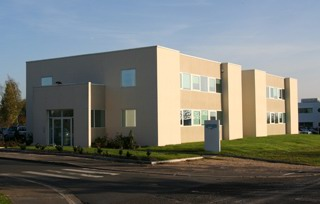
\includegraphics[scale=0.5]{../images/siege_interlog.jpg}
%	\caption{Siège social, Interlog Services à Orléans}
%	\label{Siege interlog}
%\end{figure}

\mysection{Interlog Services}

\begin{photo}[!h]
	\centering
	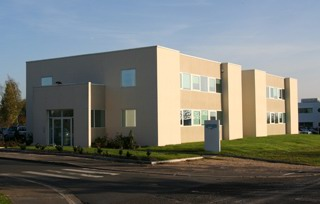
\includegraphics[scale=0.5]{../images/siege_interlog.jpg}
	\caption{Siège social, Interlog Services à Orléans}
\end{photo}

\mysubsection{Présentation de l'entreprise}
\textit{Interlog Service}, anciennement \textit{ipseurope}, a été créé en 1999. Il s'agit de la première société à proposer sur le continent européen des audits de factures de transport.\\

La société intervient au coeur de la \og Supply-Chain\fg \footnote{chaîne logistique}  et propose des prestations permettant des gains non négligeables. Les clients viennent de tous les secteurs d'activités (luxe, agroalimentaire, automobile \ldots).

\mysubsection{La direction}
L'équipe de direction est composée :
\begin{itemize}
\item d'un président,
\item d'une directrice générale et d'un directeur général,
\item d'un directeur commercial,
\item d'un directeur des opérations logistiques,
\item d'un directeur informatique.
\end{itemize}

\mysubsection{Le secteur informatique}
Le secteur informatique est dirigé par le directeur informatique, Monsieur Zoïs. L'équipe de développeurs informatiques est composée de six personnes dont le chef de projets et  cinq développeurs.\\

Le but principal de cette équipe est de développer des applications, elle  met également à jour celles  existant déjà, et règle d'éventuels bugs informatiques. Elle peut aussi, en fonction de la demande du client,  développer de nouvelles fonctionnalités nécessaires à ce dernier.